\documentclass[../main/Notes.tex]{subfiles}
\begin{document}

\section[Probability Refresher I]{Probability Refresher I \iftoggle{showdates}{\small{\textit{2014-04-22}}}{}}

\subsection*{What is Logic? What is Probability Theory?}

\textbf{Logic}\index{Logic} is reasoning under certainty, \textbf{Probability Theory}\index{Probability Theory} is reasoning under uncertainty. In Logic we can distinguish between descriptive and prescriptive approaches - in Probability Theory we distinguish between the frequentist and the Bayesian view.

The two views in Probability Theory are different in how probabilities are to be interpreted: The frequentist view interprets probabilities as \textbf{limits of relative frequencies}, while the Bayesian view interprets probabilities as \textbf{beliefs}. This course will try to make the distinction between both views clear.

\begin{figure}[h]
     \centering
     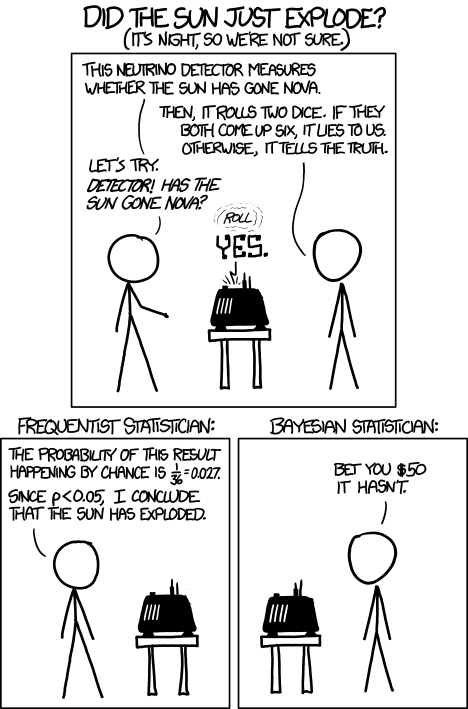
\includegraphics[scale=0.5]{../images/xkcd_frequentists_vs_bayesians}
     \caption{\textit{Source: http://xkcd.com/1132/}}
\end{figure}

\subsection{Games of Chance: Coin Toss \& Thumbtack Toss}

\subsubsection*{Coin Toss}

Alice offers Bob a bet: 
\begin{quote}
\textit{Let's toss a coin. I will give you  \$2  whenever it shows heads. But each time it shows tails, you will give me \$3.}
\end{quote}
Should Bob accept? Let's take Bob's point of view and see.
\begin{align*}
x \in \{0 = tails, 1 = heads\}\\
\mbox{If }x = 1: \mbox{Alice gives Bob \$2.}\\
\mbox{If }x = 0: \mbox{Bob gives Alice \$3.}
\end{align*}

If they play once, the money Bob gains equals: $2x - 3 (1 - x)$, with $x = 0$ on tails or $x = 1$ for heads, respectively.
But since they will play $n$ times Bob has to calculate the sum for $n$ games:
\begin{align*}
\frac{1}{n} \sum\limits_{i=1}^n \left(2x_i-3\left(1-x_i\right)\right) &= 2\left(\frac{1}{n}\sum\limits_{i=1}^n x_i\right)-3\left(\frac{1}{n}\sum\limits_{i=1}^n \left(1-x_i\right)\right)\\
&= 2\left(\frac{1}{n}\sum\limits_{i=1}^n x_i\right)-3\left(1-\frac{1}{n}\sum\limits_{i=1}^n x_i\right)
\end{align*}

Where $\frac{1}{n}\sum\limits_{i=1}^n x_i$ is the \textbf{relative proportion of heads}.\\
The expected value\index{Expected Value} (\textit{read as: ``Bob's expected gain''}) is, as can be seen above, $E = 2p - 3 (1 - p)$, where $p$ is the probability of heads.
$p$ can now easily be expressed as:
\begin{align*}
\lim_{n\rightarrow\infty}\left(\frac{1}{n}\sum\limits_{i=1}^n x_i\right) = p
\end{align*}

But what shall Bob do now, where he has a formula to derive p? Basically he has two choices: Trying out and tossing a coin $n$ times or using his \textit{a priori belief} and assigning a $p$.
How he decides is the difference between the frequentist and the Bayesian view. 
Eventually Bob sets $p = 0.5$ and inserts it into the formula for the expected outcome.
So Bob's expected gain is $E = 2 \cdot 0.5 - 3 (1 - 0.5) = -0.5 \! \left[ \$ \right] $. Hence Bob shouldn't play.

\subsubsection*{Thumbtack Toss}
\label{example:Thumbtack Toss}
Alice has another bet for Bob:
\begin{quote}
\textit{Let's toss a thumbtack. I have heads, you have tails. You are allowed to choose your stakes, but I have to agree on them to play.}
\end{quote}
What stakes should Bob choose?
We will have a look at his situation again.
\begin{align*}
x \in \{0 = tails, 1 = heads\}
\end{align*}
\begin{figure}[ht]
  \centering
  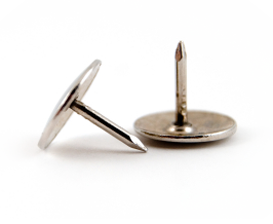
\includegraphics[scale=0.5]{../images/thumbtacks}
  \caption{Thumbtacks - left: tails, right: heads. \textit{Source: http://blog.sls-construction.com/}}
\end{figure}

The probability $p$ is again:
\begin{align*}
\lim_{n\rightarrow\infty}\left(\frac{1}{n}\sum\limits_{i=1}^n x_i\right) = p
\end{align*}

What is different is Bob's expected gain. He now has to consider the stakes as well.
\begin{align*}
E = s_1 p - s_2 (1 - p)
\end{align*}

$s_1$ is Alice's stake and $s_2$ is Bob's stake. To have a \textit{``fair''} bet the expected gain should be zero. Bob uses this knowledge to derive his stake.
\begin{align*}
& \: E = s_1 p - s_2 (1 - p)\\
0 = E \: \Leftrightarrow & \: s_1 p = s_2 (1 - p)\\
\Leftrightarrow & \: \frac{p}{1-p} = \frac{s_2}{s_1}
\end{align*}

This last formula $\frac{p}{1-p} = \frac{s_2}{s_1}$ are the \textbf{odds}\index{Odds}. If Bob fixes one stake and inserts $p$, he can calculate the other stake needed for a fair bet. But again he has the problem of how to get to $p$.

\subsubsection*{Conclusion}
To derive $p$ you always have two possibilities: The frequentist view and the Bayesian view. The difference is how we measure $p$:
\begin{itemize}
	\item \textbf{Frequentist:} measure $p$ as a property of the coin/thumbtack by throwing it $n$ times
  \item \textbf{Bayesian:} measure $p$ as a property of the ``agent'' (i.e. the decision-maker) by asking which bets are ``fair'' for him/her
\end{itemize}

\end{document}